\subsection{Conversion from Depth Image to Feature Image}\label{sec:feature_images}

The conversion of depth images to feature images needs to result in a single scalar value because all keypoint detectors work on a single signal channel.
Every feature image is calculated on range data in floating point format, potentially requiring the preprocessing step presented in Section~\ref{sec:range_depth_conversion}.
The representation change from integer to floating point data does no further processing than simple type conversion.

This section introduces and develops multiple potential feature images that were considered during this thesis.
Conversions for images of the \emph{Synthetic} scene (Section~\ref{sec:dataset_synthetic}) containing different primitive geometric structures serve as examples for the visual appeal of each feature image type.

\subsubsection{\Glspl{bearing-angle-image}}

\begin{figure}[H]
    \centering
    \tikzset{every picture/.style={line width=0.75pt}} %set default line width to 0.75pt        

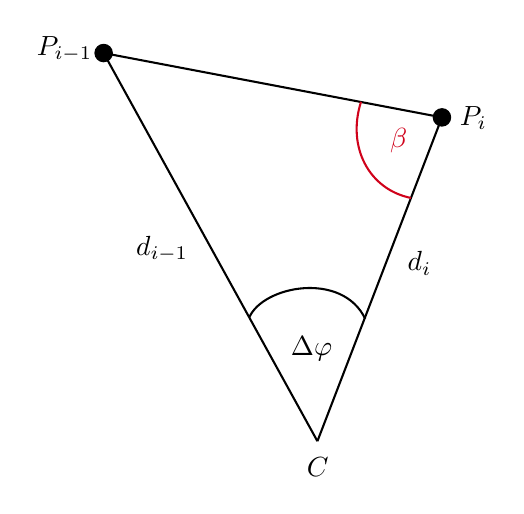
\begin{tikzpicture}[x=0.75pt,y=0.75pt,yscale=-1,xscale=1]
%uncomment if require: \path (0,227.75); %set diagram left start at 0, and has height of 227.75

%Straight Lines [id:da05017383740499093] 
\draw    (38.83,15.67) -- (141.83,202.67) ;


%Straight Lines [id:da6895513561877372] 
\draw    (201.83,46.67) -- (141.83,202.67) ;


%Curve Lines [id:da10253757735662583] 
\draw [color={rgb, 255:red, 0; green, 0; blue, 0 }  ,draw opacity=1 ]   (109,143) .. controls (115.83,127.67) and (153.83,120.67) .. (164.83,143.67) ;


%Straight Lines [id:da3851492122035306] 
\draw    (38.83,15.67) -- (201.83,46.67) ;


%Curve Lines [id:da7052636563383052] 
\draw [color={rgb, 255:red, 208; green, 2; blue, 27 }  ,draw opacity=1 ]   (162.83,39.17) .. controls (155.83,61.17) and (166.9,81.48) .. (186.9,85.48) ;


%Shape: Circle [id:dp08101382020617043] 
\draw  [fill={rgb, 255:red, 0; green, 0; blue, 0 }  ,fill opacity=1 ] (197.88,46.67) .. controls (197.88,44.49) and (199.65,42.72) .. (201.83,42.72) .. controls (204.01,42.72) and (205.78,44.49) .. (205.78,46.67) .. controls (205.78,48.85) and (204.01,50.62) .. (201.83,50.62) .. controls (199.65,50.62) and (197.88,48.85) .. (197.88,46.67) -- cycle ;
%Shape: Circle [id:dp7397482298206297] 
\draw  [fill={rgb, 255:red, 0; green, 0; blue, 0 }  ,fill opacity=1 ] (34.88,15.67) .. controls (34.88,13.49) and (36.65,11.72) .. (38.83,11.72) .. controls (41.01,11.72) and (42.78,13.49) .. (42.78,15.67) .. controls (42.78,17.85) and (41.01,19.62) .. (38.83,19.62) .. controls (36.65,19.62) and (34.88,17.85) .. (34.88,15.67) -- cycle ;


% Text Node
\draw (139,158) node [color={rgb, 255:red, 0; green, 0; blue, 0 }  ,opacity=1 ] [align=left] {$\displaystyle \Delta $$\displaystyle \varphi $};
% Text Node
\draw (181,58) node [color={rgb, 255:red, 208; green, 2; blue, 27 }  ,opacity=1 ] [align=left] {$\displaystyle \beta $};
% Text Node
\draw (191,117) node  [align=left] {$\displaystyle d_{i}$};
% Text Node
\draw (67,110) node  [align=left] {$\displaystyle d_{i-1}$};
% Text Node
\draw (217,47) node  [align=left] {$\displaystyle P_{i}$};
% Text Node
\draw (20,14) node  [align=left] {$\displaystyle P_{i-1}$};
% Text Node
\draw (142,215) node  [align=left] {$\displaystyle C$};


\end{tikzpicture}
%
    \caption[Schematic Representation of Bearing-Angles]{This figure shows the relationship of the light rays that form the \gls{bearing-angle} $\beta$.}\label{fig:bearing_angle}
\end{figure}

Scaramuzza et.al\cite{Scaramuzza2007} proposes \Glspl{bearing-angle-image} were each pixel is the angle between the current point, the optical center and the previous point.
Lin et.al\cite{Lin2017} use \Glspl{bearing-angle-image} to automatically align pointclouds using keypoints extracted with \acrshort{surf}.
Figure~\ref{fig:bearing_angle} shows the triangle that these three points form.
The neighbourhood relationship can be choosen arbitrarily resulting in four \Glspl{bearing-angle-image}, horizontal, vertical, diagonal and antidiagonal.
The second variable is the direction the angle is calculted, e.g.~for horizontal images it can be calculated from left-to-right or right-to-left.
This does not exhibit new information, because the angle of the other direction is immediatly known from the fact that the sum of the angles is $180\degree$.
Nontheless, the direction must be defined to obtain stable visual features.

The formula for the \gls{bearing-angle} $\beta$ is derived with the cosine theorem.
For the horizontal left-to-right calculation the formula is as follows.
\begin{equation}
    \beta = \arccos%
            \frac{d_{i,j} - d_{i-1,j} \cos \Delta\varphi}%
                 {\sqrt{d_{i,j}^2 + d_{i-1,j}^2 - 2 d_{i,j} d_{i-1,j} \cos \Delta\varphi}}
\end{equation}
Note that both Scaramuzza\cite{Scaramuzza2007} and Lin\cite{Lin2017} have typos in the formulae they provided.
A full derivation for the correct equation is provided in Appendix~\ref{sec:bearing_derivation}.

The angular resolution $d\varphi$ between two pixels of the depth image depends on the camera model in use.
The pinhole models angular resolution changes between pixel pairs, equirectangular image have a constant resolution between pixels.
In general, the angle $d\varphi$ can be calculated with the spherical coordinates $P_{\mathcal{S},1}, P_{\mathcal{S},2}$ of the pixel pair $p_1, p_2$.
\begin{equation}
\begin{aligned}
    \abs{\vec{P_{\mathcal{S},1}}} &= \abs{\vec{P_{\mathcal{S},2}}} = 1 \implies P_{\mathcal{S},1} \cdot P_{\mathcal{S},2} = \cos d\varphi \\
    d\varphi &= \arccos P_{\mathcal{S},1} \cdot P_{\mathcal{S},2}
\end{aligned}
\end{equation}

The \Gls{bearing-angle} is in the range $\beta \in (0, \pi)~rad$.
Linear scaling of the angle to the color depth of the target image results in a grayscale image suitable for feature extraction.
A general scaling function for an \emph{unsigned 8bit} image and arbitrary angle range follows here.
This formulation can be used for different color depths and other potential angle calculations that result in different boundary conditions.
\begin{equation}
\begin{aligned}
    \beta_{min} &= 0 ~& c_{min} &= 0 \\
    \beta_{max} &= \pi ~& c_{max} &= 255 \\
    \beta_{scaled} &= \floor*{c_{min} + \beta \frac{c_{max} - c_{min}}{\beta_{max} - \beta_{min}}}
\end{aligned}
\end{equation}

\subsubsection*{Characteristics}

\begin{figure}[H]
    \begin{subfigure}[t]{0.32\textwidth}
        \includegraphics[width=\linewidth]{chapter04/img/bearing-diag-0001.png}
        \caption{This figure shows a converted \gls{bearing-angle-image} on a synthetic rendered scene.}
    \end{subfigure}
    \begin{subfigure}[t]{0.32\textwidth}
        \includegraphics[width=\linewidth]{chapter04/img/bearing-diag-0030.png}
        \caption{Rotating the camera demonstrates color changes of surfaces.}
    \end{subfigure}
    \begin{subfigure}[t]{0.32\textwidth}
        \includegraphics[width=\linewidth]{chapter04/img/bearing-diag-0210.png}
        \caption{A different camera pose result in different surface shading.}
    \end{subfigure}
    \caption[Bearing Angle Image Characteristics demonstrated]{The \gls{bearing-angle-image} is not invariant to rotation and viewpoint changes. This property limits its applicability for automatic registration of bigger discontinues changes of the camera pose. Each depth image was converted with the diagonal (topleft-to-bottom-right direction) implementation of the \gls{bearing-angle} formula.}
\end{figure}

\subsubsection{Multi-Directional Bearing Angle}

The \gls{max-curve-image} tries generalize the \gls{bearing-angle} to be rotation invariant as it takes the \gls{bearing-angle} in each direction into account.
Additionally to the left-sided \gls{bearing-angle} the right-sided angle is calculated as well and finally added.

\begin{figure}
    

\tikzset{every picture/.style={line width=0.75pt}} %set default line width to 0.75pt        

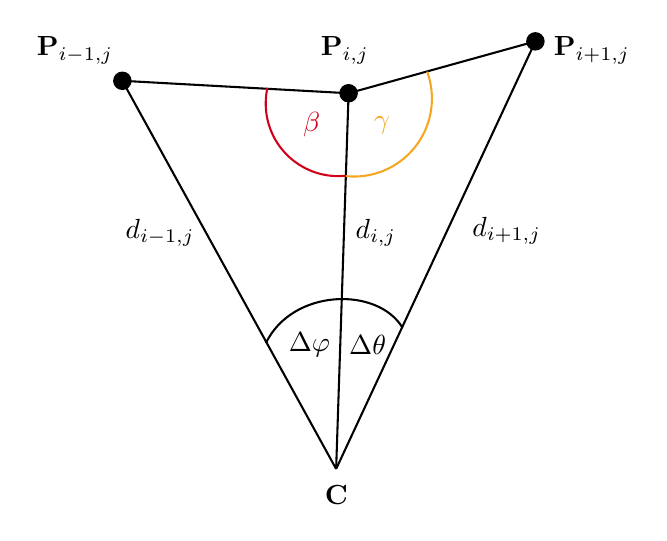
\begin{tikzpicture}[x=0.75pt,y=0.75pt,yscale=-1,xscale=1]
%uncomment if require: \path (0,252); %set diagram left start at 0, and has height of 252

%Straight Lines [id:da05017383740499093] 
\draw    (46.83,26.67) -- (149.83,213.67) ;
%Straight Lines [id:da6895513561877372] 
\draw    (155.83,32.67) -- (149.83,213.67) ;
%Curve Lines [id:da10253757735662583] 
\draw [color={rgb, 255:red, 0; green, 0; blue, 0 }  ,draw opacity=1 ]   (116,153) .. controls (128.83,126.67) and (169.83,125.67) .. (181.83,145.67) ;
%Straight Lines [id:da3851492122035306] 
\draw    (46.83,26.67) -- (155.83,32.67) ;
%Shape: Circle [id:dp08101382020617043] 
\draw  [fill={rgb, 255:red, 0; green, 0; blue, 0 }  ,fill opacity=1 ] (151.88,32.67) .. controls (151.88,30.49) and (153.65,28.72) .. (155.83,28.72) .. controls (158.01,28.72) and (159.78,30.49) .. (159.78,32.67) .. controls (159.78,34.85) and (158.01,36.62) .. (155.83,36.62) .. controls (153.65,36.62) and (151.88,34.85) .. (151.88,32.67) -- cycle ;
%Shape: Circle [id:dp7397482298206297] 
\draw  [fill={rgb, 255:red, 0; green, 0; blue, 0 }  ,fill opacity=1 ] (42.88,26.67) .. controls (42.88,24.49) and (44.65,22.72) .. (46.83,22.72) .. controls (49.01,22.72) and (50.78,24.49) .. (50.78,26.67) .. controls (50.78,28.85) and (49.01,30.62) .. (46.83,30.62) .. controls (44.65,30.62) and (42.88,28.85) .. (42.88,26.67) -- cycle ;
%Shape: Circle [id:dp7936487176657823] 
\draw  [fill={rgb, 255:red, 0; green, 0; blue, 0 }  ,fill opacity=1 ] (241.88,7.67) .. controls (241.88,5.49) and (243.65,3.72) .. (245.83,3.72) .. controls (248.01,3.72) and (249.78,5.49) .. (249.78,7.67) .. controls (249.78,9.85) and (248.01,11.62) .. (245.83,11.62) .. controls (243.65,11.62) and (241.88,9.85) .. (241.88,7.67) -- cycle ;
%Straight Lines [id:da7225304487809803] 
\draw    (245.83,7.67) -- (149.83,213.67) ;
%Straight Lines [id:da15289701870660388] 
\draw    (155.83,32.67) -- (245.83,7.67) ;
%Shape: Arc [id:dp845909277560968] 
\draw  [draw opacity=0] (154.29,72.43) .. controls (153.16,72.54) and (152.02,72.6) .. (150.87,72.6) .. controls (131.56,72.6) and (115.9,56.94) .. (115.9,37.63) .. controls (115.9,35.08) and (116.17,32.59) .. (116.69,30.19) -- (150.87,37.63) -- cycle ; \draw  [color={rgb, 255:red, 208; green, 2; blue, 27 }  ,draw opacity=1 ] (154.29,72.43) .. controls (153.16,72.54) and (152.02,72.6) .. (150.87,72.6) .. controls (131.56,72.6) and (115.9,56.94) .. (115.9,37.63) .. controls (115.9,35.08) and (116.17,32.59) .. (116.69,30.19) ;
%Shape: Arc [id:dp15343497156889918] 
\draw  [draw opacity=0] (193.67,22.29) .. controls (195.16,26.33) and (195.97,30.7) .. (195.97,35.25) .. controls (195.97,55.99) and (179.15,72.8) .. (158.42,72.8) .. controls (157.06,72.8) and (155.72,72.73) .. (154.4,72.59) -- (158.42,35.25) -- cycle ; \draw  [color={rgb, 255:red, 245; green, 166; blue, 35 }  ,draw opacity=1 ] (193.67,22.29) .. controls (195.16,26.33) and (195.97,30.7) .. (195.97,35.25) .. controls (195.97,55.99) and (179.15,72.8) .. (158.42,72.8) .. controls (157.06,72.8) and (155.72,72.73) .. (154.4,72.59) ;

% Text Node
\draw (137,154) node  [color={rgb, 255:red, 0; green, 0; blue, 0 }  ,opacity=1 ] [align=left] {$\displaystyle \Delta $$\displaystyle \varphi $};
% Text Node
\draw (138,48) node  [color={rgb, 255:red, 208; green, 2; blue, 27 }  ,opacity=1 ] [align=left] {$\displaystyle \beta $};
% Text Node
\draw (169,100) node   [align=left] {$\displaystyle d_{i,j}$};
% Text Node
\draw (65,100) node   [align=left] {$\displaystyle d_{i-1,j}$};
% Text Node
\draw (154,12) node   [align=left] {$\displaystyle \mathbf{P}_{i,j}$};
% Text Node
\draw (150,226) node   [align=left] {$\displaystyle \mathbf{C}$};
% Text Node
\draw (232,99) node   [align=left] {$\displaystyle d_{i+1,j}$};
% Text Node
\draw (172,48) node   [align=left] {$\displaystyle \textcolor[rgb]{0.96,0.65,0.14}{\gamma }$};
% Text Node
\draw (165,154) node  [color={rgb, 255:red, 0; green, 0; blue, 0 }  ,opacity=1 ] [align=left] {$\displaystyle \Delta $$\displaystyle \theta $};
% Text Node
\draw (273,12) node   [align=left] {$\displaystyle \mathbf{P}_{i+1,j}$};
% Text Node
\draw (24,12) node   [align=left] {$\displaystyle \mathbf{P}_{i-1,j}$};


\end{tikzpicture}


    \caption[Schematic Representation of the Max-Curve]{The Max-Curve composes two \Glspl{bearing-angle} in vertical, horizontal, diagonal and antidiagonal direction. The maximum angle is then selected as pixel value.}
\end{figure}

This makes the measure more robust to rotation, but does not produce good features.
\begin{align}
    B &= \max{\{B_{diagonal}, B_{antidiagonal}, B_{horizontal}, B_{vertical}\}}
\end{align}

\begin{figure}[H]
    \begin{subfigure}[t]{0.32\textwidth}
        \includegraphics[width=\linewidth]{chapter04/img/max-0001.png}
        \caption{This figure shows a converted \gls{bearing-angle-image} on a synthetic rendered scene.}
    \end{subfigure}
    \begin{subfigure}[t]{0.32\textwidth}
        \includegraphics[width=\linewidth]{chapter04/img/max-0030.png}
        \caption{Rotating the camera demonstrates color changes of surfaces.}
    \end{subfigure}
    \begin{subfigure}[t]{0.32\textwidth}
        \includegraphics[width=\linewidth]{chapter04/img/max-0210.png}
        \caption{A different camera pose result in different surface shading.}
    \end{subfigure}
\end{figure}

\subsubsection{Curvature}

\begin{figure}[H]
    \begin{subfigure}[t]{0.47\textwidth}
        \scalebox{0.9}{%
        \begin{tikzpicture}
\begin{axis}[xmin=-0.7,
             xmax=0.7,
             ymin=-0.1,
             ymax=1.1,
             samples=200,
             axis line style={draw=none},
             tick style={draw=none},
             xticklabels={\empty},
             yticklabels={\empty},
             grid=major,
             plot box ratio={2 1},
             axis equal]
    \draw[plotorange, line width=1.3pt] (axis cs:0,0.5) circle [radius=50];
    \addplot[plotblue, line width=1.5pt] {x*x};
    \coordinate (C) at (axis cs:{0.0,0.5});
    \coordinate (O) at (axis cs:{0.0,0.0});
    \coordinate (L) at (axis cs:{0.1,0.25});
    \node at (L) {$\mathbf{r}$};
    \node[label={90:{$\mathbf{C}$}},circle,fill,inner sep=1pt] at (C) {};
    \draw[thick,-](C)--(O);
\end{axis}
\end{tikzpicture}

        }
        \caption{The curvature of a line at a specific point is defined through its osculating circle.}
    \end{subfigure}
    \begin{subfigure}[t]{0.47\textwidth}
        \scalebox{0.9}{%
        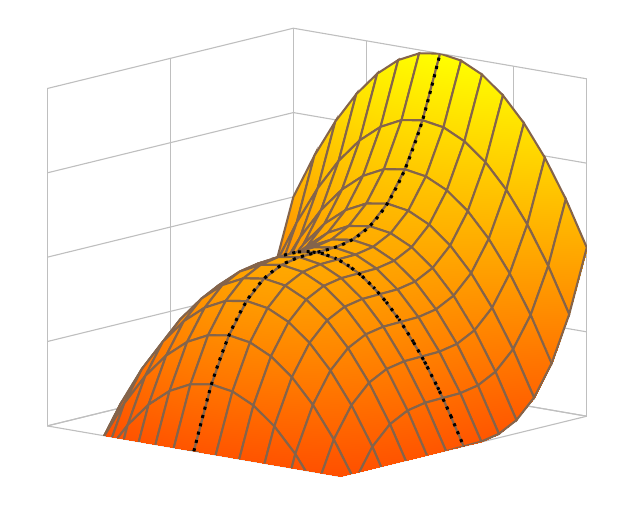
\begin{tikzpicture}
\begin{axis}[xmin=-1.0,xmax=1.0,
             ymin=-1.0,ymax=1.0,
             zmin=-1.0,zmax=1.0,
             grid=major,
             axis line style={draw=none},
             tick style={draw=none},
             view={310}{35},
             xticklabels={\empty},
             yticklabels={\empty},
             zticklabels={\empty},
             plot box ratio={1 1 3},
             colormap/redyellow]
\newcommand\func[2]{#1^3 - #2^2}
\definecolor{darkorange}{HTML}{84644B}

    \addplot3[surf,
              shader=faceted interp,
              faceted color={darkorange},
              samples=15,
              domain=-1:1,
              y domain=-1:1] {\func{x}{y}};

    % plot curve for x direction
    \addplot3[samples=15,
              domain=-1:1,
              samples y=1,
              dotted,
              black,
              line width=1.1pt,
              smooth] (x, 0, \func{x}{0});
    % plot curve for y direction
    \addplot3[samples=15,
              domain=-1:1,
              y domain=-1:0.22,
              dotted,
              black,
              line width=1.1pt,
              smooth] (0, y, \func{0}{y});
\end{axis}
\end{tikzpicture}

        }
        \caption{The curvature of a surface at a given point depends on the direction of measurement. The principal curvatures are the maximum and minimum value of curvatures in all directions.}
    \end{subfigure}
\end{figure}

As a different analytical approach to producing feature images the calculation of the \gls{curvature} for each depth value.
The two common measures of curvature in differential geometry are \gls{gaussian-curvature} and \gls{mean-curvature}\cite{Kuhnel2008}.

If the function is known as a graph the \Gls{gaussian-curvature} can be estimated using the derivatives of the function.
For depth data each depth value is a sample of this function graph and numeric approximation of the derivatives allows the calculation of the curvature.
\begin{align}
    \mathfrak{K} &= \frac{f_{uu} f_{vv} - f_{uv}^2}{{(1 + f_u^2 + f_v^2)}^2}
\end{align}
With
\begin{align*}
    f_{x} &= \frac{y_1 - y_0}{\Delta x} \\
    f_{xx} &= \frac{y_1 + y_{-1} - 2 y_0}{{\Delta x}^2}
\end{align*}
as approximation for the derivatives.

Similarly, the \Gls{mean-curvature} can be calculated with a different formula.
\begin{align}
    \mathfrak{H} &= \frac{{(1 + f_{v}^2)} f_{uu} - 2 f_u f_v f_{uv} + {(1 + f_u^2)} f_{vv}}{2 \sqrt{1 + f_u^2 + f_v^2}^3}
\end{align}
Both measures of curvature are $\mathfrak{K},\mathfrak{H} \in {\rm I\!R}$.
To convert them into a meaningful grayscale image they need to be clamped to arbitrary bounds, that can be choosen based on visual distinctiveness or other heuristics.
After clamping the values are scaled and quantized accordingly.

\subsubsection{\Glspl{flexion-image}}\label{flexion-image-section}

The local shape of an object that is sampled by a depth sensor is characterized by its normalized surface normal.
A surface normal is a vector perpendicular to the surface of the object.
This characterization builds the foundation of the \Gls{flexion-image} and its inspiration, too.

Each measured pixel is backprojected to camera coordinates, scaling the point in spherical coordinates with its measured range, as first step.
Approximating the normal for a measured surface point $\mathbf{P_{i,j}}$ is possible using the cross product of its neighbours connecting vectors.
The point relationship is visualized in Figure~\ref{fig:flexion_normals_plane}.
\begin{figure}[H]
    \begin{subfigure}[t]{0.49\linewidth}
        \centering
        \scalebox{1.0}{%
        

\tikzset{every picture/.style={line width=0.75pt}} %set default line width to 0.75pt        

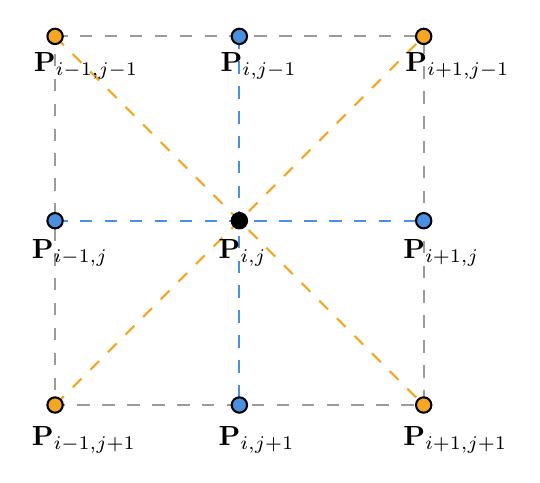
\begin{tikzpicture}[x=0.75pt,y=0.75pt,yscale=-1,xscale=1]
%uncomment if require: \path (0,237); %set diagram left start at 0, and has height of 237

%Shape: Rectangle [id:dp6565487036659107] 
\draw  [color={rgb, 255:red, 155; green, 155; blue, 155 }  ,draw opacity=1 ][dash pattern={on 4.5pt off 4.5pt}] (28.7,13.7) -- (206.3,13.7) -- (206.3,191.3) -- (28.7,191.3) -- cycle ;
%Straight Lines [id:da30195081571029425] 
\draw [color={rgb, 255:red, 74; green, 144; blue, 226 }  ,draw opacity=1 ] [dash pattern={on 4.5pt off 4.5pt}]  (28.7,102.5) -- (206.3,102.5) ;
%Straight Lines [id:da4586174781414081] 
\draw [color={rgb, 255:red, 74; green, 144; blue, 226 }  ,draw opacity=1 ] [dash pattern={on 4.5pt off 4.5pt}]  (117.5,13.7) -- (117.5,191.3) ;
%Straight Lines [id:da7294828306266232] 
\draw [color={rgb, 255:red, 245; green, 166; blue, 35 }  ,draw opacity=1 ] [dash pattern={on 4.5pt off 4.5pt}]  (28.7,13.7) -- (206.3,191.3) ;
%Straight Lines [id:da3243995266948473] 
\draw [color={rgb, 255:red, 245; green, 166; blue, 35 }  ,draw opacity=1 ] [dash pattern={on 4.5pt off 4.5pt}]  (28.7,191.3) -- (206.3,13.7) ;
%Shape: Circle [id:dp5266363779447065] 
\draw  [fill={rgb, 255:red, 245; green, 166; blue, 35 }  ,fill opacity=1 ] (25,13.7) .. controls (25,11.66) and (26.66,10) .. (28.7,10) .. controls (30.74,10) and (32.4,11.66) .. (32.4,13.7) .. controls (32.4,15.74) and (30.74,17.4) .. (28.7,17.4) .. controls (26.66,17.4) and (25,15.74) .. (25,13.7) -- cycle ;
%Shape: Ellipse [id:dp14497174740803043] 
\draw  [fill={rgb, 255:red, 74; green, 144; blue, 226 }  ,fill opacity=1 ] (25,102.5) .. controls (25,100.46) and (26.66,98.8) .. (28.7,98.8) .. controls (30.74,98.8) and (32.4,100.46) .. (32.4,102.5) .. controls (32.4,104.54) and (30.74,106.2) .. (28.7,106.2) .. controls (26.66,106.2) and (25,104.54) .. (25,102.5) -- cycle ;
%Shape: Ellipse [id:dp0427609892023727] 
\draw  [fill={rgb, 255:red, 245; green, 166; blue, 35 }  ,fill opacity=1 ] (25,191.3) .. controls (25,189.26) and (26.66,187.6) .. (28.7,187.6) .. controls (30.74,187.6) and (32.4,189.26) .. (32.4,191.3) .. controls (32.4,193.34) and (30.74,195) .. (28.7,195) .. controls (26.66,195) and (25,193.34) .. (25,191.3) -- cycle ;
%Shape: Ellipse [id:dp2872052196845898] 
\draw  [fill={rgb, 255:red, 74; green, 144; blue, 226 }  ,fill opacity=1 ] (113.8,13.7) .. controls (113.8,11.66) and (115.46,10) .. (117.5,10) .. controls (119.54,10) and (121.2,11.66) .. (121.2,13.7) .. controls (121.2,15.74) and (119.54,17.4) .. (117.5,17.4) .. controls (115.46,17.4) and (113.8,15.74) .. (113.8,13.7) -- cycle ;
%Shape: Circle [id:dp758793708555806] 
\draw  [fill={rgb, 255:red, 0; green, 0; blue, 0 }  ,fill opacity=1 ] (113.8,102.5) .. controls (113.8,100.46) and (115.46,98.8) .. (117.5,98.8) .. controls (119.54,98.8) and (121.2,100.46) .. (121.2,102.5) .. controls (121.2,104.54) and (119.54,106.2) .. (117.5,106.2) .. controls (115.46,106.2) and (113.8,104.54) .. (113.8,102.5) -- cycle ;
%Shape: Circle [id:dp477059334030714] 
\draw  [fill={rgb, 255:red, 74; green, 144; blue, 226 }  ,fill opacity=1 ] (113.8,191.3) .. controls (113.8,189.26) and (115.46,187.6) .. (117.5,187.6) .. controls (119.54,187.6) and (121.2,189.26) .. (121.2,191.3) .. controls (121.2,193.34) and (119.54,195) .. (117.5,195) .. controls (115.46,195) and (113.8,193.34) .. (113.8,191.3) -- cycle ;
%Shape: Ellipse [id:dp13207731000753575] 
\draw  [fill={rgb, 255:red, 245; green, 166; blue, 35 }  ,fill opacity=1 ] (202.6,13.7) .. controls (202.6,11.66) and (204.26,10) .. (206.3,10) .. controls (208.34,10) and (210,11.66) .. (210,13.7) .. controls (210,15.74) and (208.34,17.4) .. (206.3,17.4) .. controls (204.26,17.4) and (202.6,15.74) .. (202.6,13.7) -- cycle ;
%Shape: Circle [id:dp8288145253462365] 
\draw  [fill={rgb, 255:red, 74; green, 144; blue, 226 }  ,fill opacity=1 ] (202.6,102.5) .. controls (202.6,100.46) and (204.26,98.8) .. (206.3,98.8) .. controls (208.34,98.8) and (210,100.46) .. (210,102.5) .. controls (210,104.54) and (208.34,106.2) .. (206.3,106.2) .. controls (204.26,106.2) and (202.6,104.54) .. (202.6,102.5) -- cycle ;
%Shape: Circle [id:dp9160642610677009] 
\draw  [fill={rgb, 255:red, 245; green, 166; blue, 35 }  ,fill opacity=1 ] (202.6,191.3) .. controls (202.6,189.26) and (204.26,187.6) .. (206.3,187.6) .. controls (208.34,187.6) and (210,189.26) .. (210,191.3) .. controls (210,193.34) and (208.34,195) .. (206.3,195) .. controls (204.26,195) and (202.6,193.34) .. (202.6,191.3) -- cycle ;

% Text Node
\draw (106,110) node [anchor=north west][inner sep=0.75pt]   [align=left] {$\displaystyle \mathbf{P}_{i,j}$};
% Text Node
\draw (195,110) node [anchor=north west][inner sep=0.75pt]   [align=left] {$\displaystyle \mathbf{P}_{i+1,j}$};
% Text Node
\draw (16,110) node [anchor=north west][inner sep=0.75pt]   [align=left] {$\displaystyle \mathbf{P}_{i-1,j}$};
% Text Node
\draw (107,20) node [anchor=north west][inner sep=0.75pt]   [align=left] {$\displaystyle \mathbf{P}_{i,j-1}$};
% Text Node
\draw (196,20) node [anchor=north west][inner sep=0.75pt]   [align=left] {$\displaystyle \mathbf{P}_{i+1,j-1}$};
% Text Node
\draw (17,20) node [anchor=north west][inner sep=0.75pt]   [align=left] {$\displaystyle \mathbf{P}_{i-1,j-1}$};
% Text Node
\draw (106,200) node [anchor=north west][inner sep=0.75pt]   [align=left] {$\displaystyle \mathbf{P}_{i,j+1}$};
% Text Node
\draw (195,200) node [anchor=north west][inner sep=0.75pt]   [align=left] {$\displaystyle \mathbf{P}_{i+1,j+1}$};
% Text Node
\draw (16,200) node [anchor=north west][inner sep=0.75pt]   [align=left] {$\displaystyle \mathbf{P}_{i-1,j+1}$};


\end{tikzpicture}


        }
        \caption{The normals for a point $\mathbf{P_{i,j}}$ can be estimated its diagonal or horizontal and vertical neighbours.}\label{fig:flexion_normals_plane}
    \end{subfigure}
    \begin{subfigure}[t]{0.49\linewidth}
        \centering
        \begin{tikzpicture}
    \node[anchor=south west,inner sep=0] (image) at (4.0,0) {\includegraphics[width=0.6\textwidth]{chapter04/img/flexion-model-2-clipped.png}};
    \node at (4.4, 5.1) {$\mathbf{P_{i-1,j-1}}$};
    \node at (6.2, 5.5) {$\mathbf{P_{i,j-1}}$};
    \node at (8.5, 5.8) {$\mathbf{P_{i+1,j-1}}$};

    \node at (4.7, 2.9) {\scalebox{0.9}{$\mathbf{P_{i-1,j}}$}};
    \node at (6.2, 2.5) {$\mathbf{P_{i,j}}$};
    \node at (7.7, 3.0) {$\mathbf{P_{i+1,j}}$};

    \node at (5.0, 0.9) {$\mathbf{P_{i-1,j+1}}$};
    \node at (6.3, 0.4) {$\mathbf{P_{i,j+1}}$};
    \node at (9.2, 0.3) {$\mathbf{P_{i+1,j+1}}$};

    \node [plotdarkblue] at (4.6, 3.5) {$\vec{n_1}$};
    \node [plotdarkorange] at (4.8, 2.3) {$\vec{n_2}$};
\end{tikzpicture}

        \caption{The estimated normals span an angle depending on the local shape of the surface measured by the depth sensors.}\label{fig:flexion_space}
    \end{subfigure}
    \caption[Schematic Representation of Flexion]{This figure demonstrates how flexed surfaces have different normals for diagonal and non-diagonal estimation. This difference is utilized as measure for flexion.}%
    \label{fig:flexion-image-scetched}
\end{figure}
Using the diagonal and vertical neighbouring points (blue) results a different normal than the diagonal neighbours (orange).
As Figure~\ref{fig:flexion_space} demonstrates, both normals span an angle.
\begin{equation}
\begin{aligned}
    \vec{n_1} &= \frac{\vec{P_{i,j-1}} - \vec{P_{i,j+1}}}{\lnorm{\vec{P_{i,j-1}} - \vec{P_{i,j+1}}}}
                \times \frac{\vec{P_{i-1,j}} - \vec{P_{i+1,j}}}{\lnorm{\vec{P_{i-1,j}} - \vec{P_{i+1,j}}}} \\
    \vec{n_2} &= \frac{\vec{P_{i-1,j-1}} - \vec{P_{i+1,j+1}}}{\lnorm{\vec{P_{i-1,j-1}} - \vec{P_{i+1,j+1}}}}
                \times \frac{\vec{P_{i-1,j+1}} - \vec{P_{i+1,j-1}}}{\lnorm{\vec{P_{i-1,j+1}} - \vec{P_{i+1,j-1}}}}
    \label{eq:flexion_normals}
\end{aligned}
\end{equation}
Note, that both normals $\vec{n_1}$ and $\vec{n_2}$ are not unit length, but only the direction vector between the neighbouring points of $\mathbf{P_{i,j}}$.
Finally, the Flexion $\mathcal{F}$ of point $\mathbf{P_{i,j}}$ is defined as
\begin{align}
    \mathcal{F} &= \abs{\vec{n_1} \cdotp \vec{n_2}}
\end{align}
Because $\lnorm{\vec{n_1}},\lnorm{\vec{n_2}} \in [0,1]$ the value of is bound to $\mathcal{F} \in [0, 1]$.
Creating the final image requires a linear scaling to the desired output image depth using Equation~\ref{eq:linear_scaling}.

Figure~\ref{fig:flexion_images} visualizes the \Gls{flexion-image} for the same camera positions as for the other feature images.
\begin{figure}[H]
    \begin{subfigure}[t]{0.32\textwidth}
        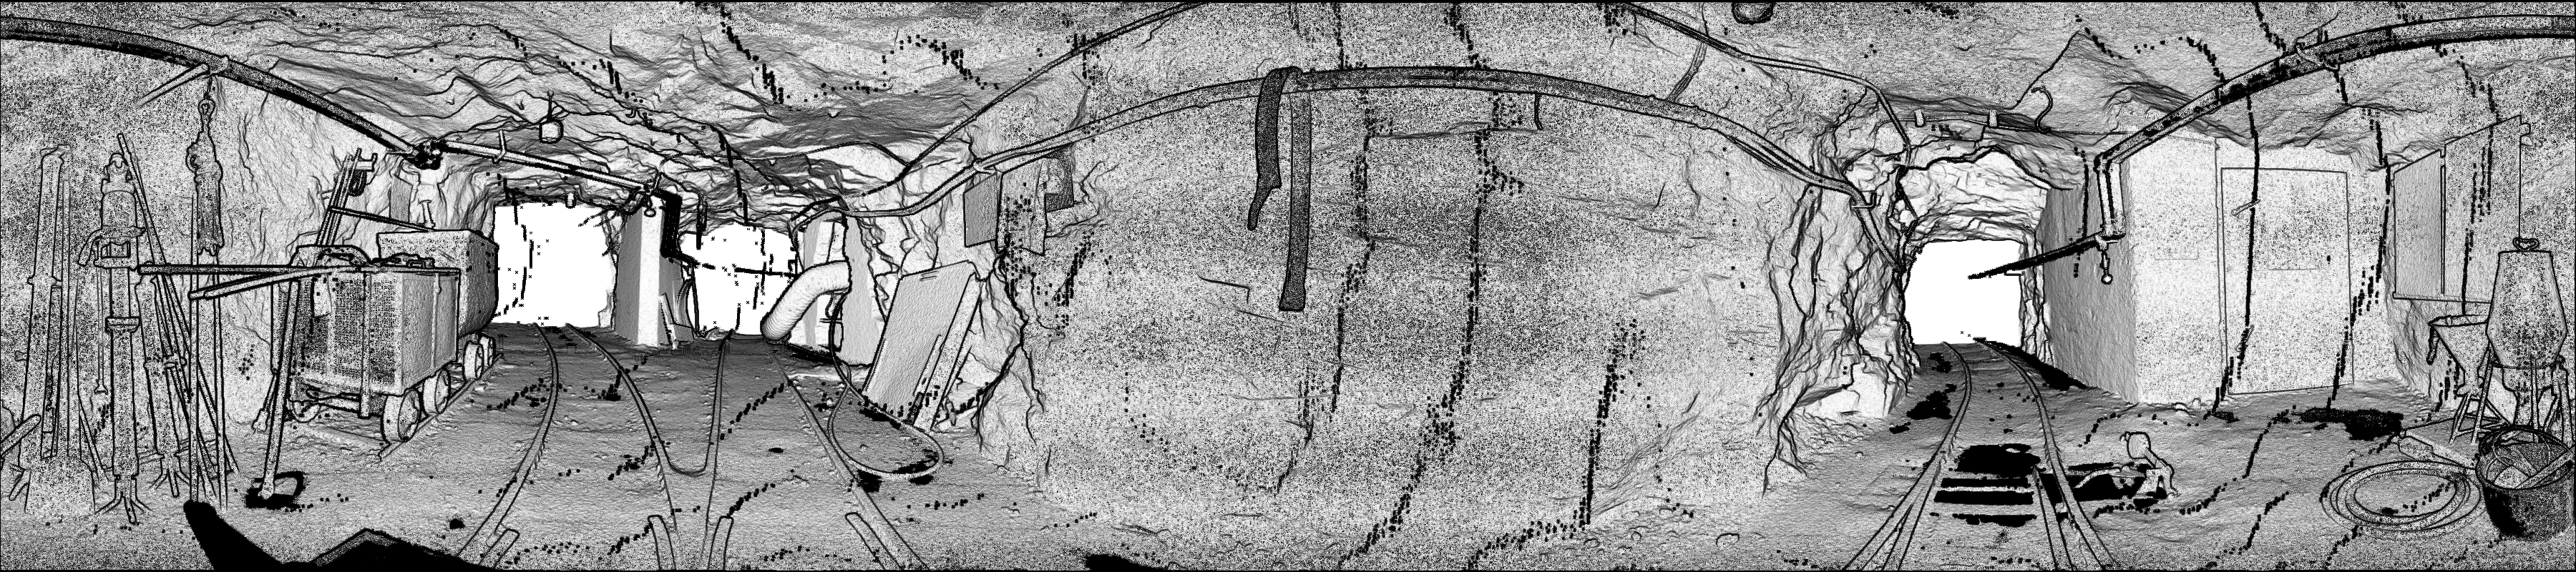
\includegraphics[width=\linewidth]{chapter04/img/flexion-0001.png}
        \caption{}
    \end{subfigure}
    \begin{subfigure}[t]{0.32\textwidth}
        \includegraphics[width=\linewidth]{chapter04/img/flexion-0030.png}
        \caption{}
    \end{subfigure}
    \begin{subfigure}[t]{0.32\textwidth}
        \includegraphics[width=\linewidth]{chapter04/img/flexion-0210.png}
        \caption{}
    \end{subfigure}
    \caption{These figures demonstrate the characteristical look of the \Glspl{flexion-image}. Its appearence is very plastic and the shading effects give a good feel for depth. The conversion is rotation invariant.}\label{fig:flexion_images}
\end{figure}

\subsubsection*{Characteristics}

The \gls{flexion-image} is rotation invariant.
Rotation of either an object or the camera does not change the difference between the two normal approximations.
A flat surface has an almost constant shading, because the normal approximation results in the same vector directions.
Flat surfaces not perpendicular to the camera plane have non-constant shading with the brightness reduced the further the surface patch is appart from the camera center.
This effect is caused by the perspective transformation.
The length of the normal vectors reduces with the distance to the camera, because the diagonals gets smaller, as Figure~\ref{fig:flexion_angle_decrease} demonstrates.
\begin{figure}[H]
    

\tikzset{every picture/.style={line width=0.75pt}} %set default line width to 0.75pt        

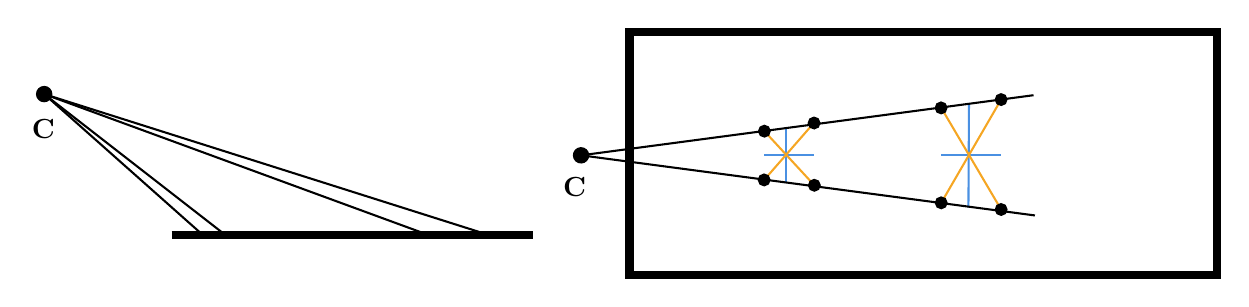
\begin{tikzpicture}[x=0.75pt,y=0.75pt,yscale=-1,xscale=1]
%uncomment if require: \path (0,142); %set diagram left start at 0, and has height of 142

%Straight Lines [id:da6840514143989631] 
\draw [color={rgb, 255:red, 74; green, 144; blue, 226 }  ,draw opacity=1 ]   (366.4,69.04) -- (390.44,69.04) ;
%Straight Lines [id:da9689027017272559] 
\draw [color={rgb, 255:red, 74; green, 144; blue, 226 }  ,draw opacity=1 ]   (377.02,82.13) -- (377.02,55.88) ;
%Straight Lines [id:da8683032061954556] 
\draw [color={rgb, 255:red, 74; green, 144; blue, 226 }  ,draw opacity=1 ]   (451.65,69.04) -- (480.52,69.04) ;
%Straight Lines [id:da6934594327602702] 
\draw [color={rgb, 255:red, 74; green, 144; blue, 226 }  ,draw opacity=1 ]   (464.75,94.04) -- (465.02,44.04) ;
%Straight Lines [id:da7261021710957941] 
\draw [color={rgb, 255:red, 245; green, 166; blue, 35 }  ,draw opacity=1 ]   (480.5,42.14) -- (451.64,91.89) ;
%Straight Lines [id:da37992799055918147] 
\draw [color={rgb, 255:red, 245; green, 166; blue, 35 }  ,draw opacity=1 ]   (451.58,46) -- (480.5,95.1) ;
%Straight Lines [id:da15457235634391941] 
\draw [color={rgb, 255:red, 245; green, 166; blue, 35 }  ,draw opacity=1 ]   (389.38,54.43) -- (366.33,80.86) ;
%Straight Lines [id:da05878950535382432] 
\draw [color={rgb, 255:red, 245; green, 166; blue, 35 }  ,draw opacity=1 ]   (366.45,57.36) -- (390.5,83.43) ;
%Straight Lines [id:da045550454885305736] 
\draw [line width=3]    (80.9,107.5) -- (254.9,107.5) ;
%Shape: Circle [id:dp8549507101465224] 
\draw  [fill={rgb, 255:red, 0; green, 0; blue, 0 }  ,fill opacity=1 ] (16,39.5) .. controls (16,37.59) and (17.54,36.05) .. (19.45,36.05) .. controls (21.36,36.05) and (22.9,37.59) .. (22.9,39.5) .. controls (22.9,41.41) and (21.36,42.95) .. (19.45,42.95) .. controls (17.54,42.95) and (16,41.41) .. (16,39.5) -- cycle ;
%Straight Lines [id:da09684243305909856] 
\draw    (19.45,39.5) -- (94.9,106.5) ;
%Straight Lines [id:da4476141598512392] 
\draw    (19.45,39.5) -- (106.9,107.5) ;
%Straight Lines [id:da5555101325179832] 
\draw    (19.45,39.5) -- (204.9,107.5) ;
%Straight Lines [id:da06573307117836547] 
\draw    (19.45,39.5) -- (230.9,106.5) ;
%Shape: Circle [id:dp3195203497272404] 
\draw  [fill={rgb, 255:red, 0; green, 0; blue, 0 }  ,fill opacity=1 ] (274.67,69.08) .. controls (274.62,67.18) and (276.13,65.6) .. (278.04,65.55) .. controls (279.94,65.51) and (281.52,67.02) .. (281.57,68.92) .. controls (281.61,70.83) and (280.1,72.41) .. (278.2,72.45) .. controls (276.29,72.49) and (274.71,70.99) .. (274.67,69.08) -- cycle ;
%Straight Lines [id:da25083036265050096] 
\draw    (278.12,69) -- (496.79,97.97) ;
%Straight Lines [id:da6083860800665152] 
\draw    (278.12,69) -- (496.1,40.04) ;
%Shape: Rectangle [id:dp031034421219254926] 
\draw  [line width=3]  (301.4,9.5) -- (584.4,9.5) -- (584.4,126.5) -- (301.4,126.5) -- cycle ;
%Shape: Circle [id:dp2988386895287467] 
\draw  [fill={rgb, 255:red, 0; green, 0; blue, 0 }  ,fill opacity=1 ] (363.85,57.42) .. controls (363.81,55.99) and (364.95,54.8) .. (366.39,54.76) .. controls (367.82,54.73) and (369.01,55.87) .. (369.05,57.3) .. controls (369.08,58.74) and (367.94,59.93) .. (366.51,59.96) .. controls (365.07,60) and (363.88,58.86) .. (363.85,57.42) -- cycle ;
%Shape: Circle [id:dp49087747494377276] 
\draw  [fill={rgb, 255:red, 0; green, 0; blue, 0 }  ,fill opacity=1 ] (363.73,80.92) .. controls (363.69,79.48) and (364.83,78.29) .. (366.27,78.26) .. controls (367.7,78.23) and (368.89,79.36) .. (368.93,80.8) .. controls (368.96,82.23) and (367.82,83.42) .. (366.39,83.46) .. controls (364.95,83.49) and (363.76,82.35) .. (363.73,80.92) -- cycle ;
%Shape: Circle [id:dp3291682457892863] 
\draw  [fill={rgb, 255:red, 0; green, 0; blue, 0 }  ,fill opacity=1 ] (387.79,53.49) .. controls (387.75,52.06) and (388.89,50.87) .. (390.32,50.84) .. controls (391.76,50.8) and (392.95,51.94) .. (392.98,53.37) .. controls (393.02,54.81) and (391.88,56) .. (390.44,56.03) .. controls (389.01,56.07) and (387.82,54.93) .. (387.79,53.49) -- cycle ;
%Shape: Circle [id:dp598750640317177] 
\draw  [fill={rgb, 255:red, 0; green, 0; blue, 0 }  ,fill opacity=1 ] (387.91,83.49) .. controls (387.87,82.05) and (389.01,80.86) .. (390.44,80.83) .. controls (391.88,80.79) and (393.07,81.93) .. (393.1,83.37) .. controls (393.14,84.8) and (392,85.99) .. (390.56,86.03) .. controls (389.13,86.06) and (387.94,84.92) .. (387.91,83.49) -- cycle ;
%Shape: Circle [id:dp3156912690396848] 
\draw  [fill={rgb, 255:red, 0; green, 0; blue, 0 }  ,fill opacity=1 ] (449.04,91.95) .. controls (449.01,90.51) and (450.14,89.32) .. (451.58,89.29) .. controls (453.02,89.26) and (454.21,90.39) .. (454.24,91.83) .. controls (454.27,93.26) and (453.13,94.45) .. (451.7,94.49) .. controls (450.26,94.52) and (449.07,93.38) .. (449.04,91.95) -- cycle ;
%Shape: Circle [id:dp0381257221295519] 
\draw  [fill={rgb, 255:red, 0; green, 0; blue, 0 }  ,fill opacity=1 ] (448.99,46.21) .. controls (448.95,44.77) and (450.09,43.58) .. (451.53,43.55) .. controls (452.96,43.52) and (454.15,44.65) .. (454.18,46.09) .. controls (454.22,47.53) and (453.08,48.72) .. (451.65,48.75) .. controls (450.21,48.78) and (449.02,47.65) .. (448.99,46.21) -- cycle ;
%Shape: Circle [id:dp4047969379608699] 
\draw  [fill={rgb, 255:red, 0; green, 0; blue, 0 }  ,fill opacity=1 ] (477.91,42.2) .. controls (477.87,40.76) and (479.01,39.57) .. (480.44,39.54) .. controls (481.88,39.51) and (483.07,40.64) .. (483.1,42.08) .. controls (483.14,43.51) and (482,44.7) .. (480.56,44.74) .. controls (479.13,44.77) and (477.94,43.63) .. (477.91,42.2) -- cycle ;
%Shape: Circle [id:dp5781527725767942] 
\draw  [fill={rgb, 255:red, 0; green, 0; blue, 0 }  ,fill opacity=1 ] (477.91,95.16) .. controls (477.87,93.72) and (479.01,92.53) .. (480.44,92.5) .. controls (481.88,92.46) and (483.07,93.6) .. (483.1,95.04) .. controls (483.14,96.47) and (482,97.66) .. (480.56,97.69) .. controls (479.13,97.73) and (477.94,96.59) .. (477.91,95.16) -- cycle ;

% Text Node
\draw (12,50.05) node [anchor=north west][inner sep=0.75pt]   [align=left] {$\displaystyle \mathbf{C}$};
% Text Node
\draw (268,78.05) node [anchor=north west][inner sep=0.75pt]   [align=left] {$\displaystyle \mathbf{C}$};


\end{tikzpicture}

    \caption{The angle between the diagonals decreases with increasing distance from the camera center. This results in short normals.}\label{fig:flexion_angle_decrease}
\end{figure}
The origin is the nature of the cross product is maximal if both vectors are perpendicular.
\begin{equation*}
    \lnorm{\vec{v_1} \times \vec{v_2}} = \lnorm{\vec{v_1}} \lnorm{\vec{v_2}} \sin \angle(\vec{v_1}, \vec{v_2})
\end{equation*}
The lack of normalization in Equation~\ref{eq:flexion_normals} propagates this effect through to the scalar product.
\begin{equation*}
    \vec{v_1} \cdot \vec{v_2} = \lnorm{\vec{v_1}} \lnorm{\vec{v_2}} \cos \angle(\vec{v_1}, \vec{v_2})
\end{equation*}
This shading effect gives the \gls{flexion-image} its plastic look and helps to develop the feeling for the geometric constellations.

\subsubsection{Implementation Details}

All software developed during the thesis, including the analysis and supplementary code, are developed with rigor software engineering methods.
The library components have $100\%$ unit- and integrationtest line coverage.
Each final executable is heavily tested, too.
The overall line coverage for all project code is above $98\%$.
The implementation language is C++-17\cite{c++17} and all library depdencies use at least C++-11\cite{c++11}.
All code obeys to strong typing, design by contract\cite{meyer_ieee1992} and modern idioms of the C++ programming language\cite{stroustrup_cpppl2013}.
To uncover many runtime problems that C++ allows by its raw memory access the LLVM Address-, Memory-, Thread- and Undefined-Behaviour-Sanitizers\cite{google_sanitizers} are run over all tests.
Additional static analysis is done by clang's thread-safety analysis\cite{clang_thread_safety}, clang static analyzer\cite{clang_static_analyzer} and clang-tidy\cite{babati2017static}.
All detected issues were immediatly fixed during development.
The use of continuous integration\cite{fowler_ci2000} for the whole development cycle indicated defects within hours.

The implementation goal of the produced code is to serve as a correct reference implementation for the proposed data processing.
Therefore, no special action has been taken to improve latency or throughput of the computations.
Simple measures for speedup, namely exploiting the embarrassingly parallel nature of the processing and compiler optimizations are employed.

Each of the feature image conversions is implemented as C++ library code working on \emph{OpenCV's} \lstinline[basicstyle=\ttfamily]|cv::Mat| matrix type.
The conversion is generic in the sense, that any camera model implementing the forward and backward projection for pixel coordinates is suitable for the feature image conversion.
This genericity is achieved through the use of templates.
Type requirements are enforced with \lstinline[basicstyle=\ttfamily]|static_assert()| and concept-like\cite{c++concepts} requirement definitions.

Multiple library dependencies support the functionality of the project and shall be mentioned without a particular order.
The already mentioned \emph{opencv}\cite{opencv_library} project provides functionality for image handling and processing. 
Required types and functionality for glue-code, parallelization and general programming utilize \emph{cli11}\cite{cli11}, \emph{rang}\cite{rang}, \emph{cpp-taskflow}\cite{Huang2019CppTaskflowFT}, \emph{fmt-lib}\cite{fmtlib}, \emph{GSL}\cite{gsl}, \emph{Eigen3}\cite{eigenweb} and \emph{Boost}\cite{boost}.
Functionality and performance testing are done with \emph{doctest}\cite{doctest} and \emph{libnonius}\cite{libnonius}.
Each used revision is document in the code repository and differs between versions of the thesis code.

